% !TEX program = xelatex
\documentclass[10pt,fontset=none,twocolumn]{ctexart}
\usepackage[a4paper,top=1.8cm,bottom=1.8cm,left=1.5cm,right=1.5cm]{geometry}
\usepackage{fontspec}
\usepackage{xeCJK}
\IfFontExistsTF{SimSun}{\setCJKmainfont[BoldFont=SimHei,ItalicFont=SimSun]{SimSun}}{\setCJKmainfont{FandolSong-Regular}}
\IfFontExistsTF{SimHei}{\setCJKsansfont{SimHei}}{\setCJKsansfont{FandolHei-Regular}}
\usepackage{amsmath,amssymb,bm}
\usepackage{cite}
\usepackage{booktabs}
\usepackage{array}
\usepackage{graphicx}
\usepackage{url}
\usepackage{enumitem}
\usepackage{xcolor}
\interdisplaylinepenalty=2500

\setlength{\parskip}{0pt}
\setlength{\parindent}{2em}
\setlist[enumerate]{leftmargin=1.4em,itemsep=0pt,topsep=2pt}

\newcommand{\gsid}{\mathrm{GeoSemID}}
\newcommand{\Experts}{\mathcal{M}}
\newcommand{\POIs}{\mathcal{P}}
\newcommand{\Users}{\mathcal{U}}
\newcommand{\Train}{\mathcal{D}_{\mathrm{tr}}}
\newcommand{\HitTrain}{\mathcal{D}_{\mathrm{hit}}}
\newcommand{\Ind}{\mathbb{I}}
% \mock{...} 用于标记仍缺乏真实、可溯源来源的占位数值/论断。渲染为加粗红色，
% 以便在提交前无法被忽略；每一处 \mock{...} 都必须替换为经过验证的真实值。
\newcommand{\mock}[1]{\textbf{\textcolor{red}{#1}}}

\title{\bfseries 面向下一兴趣点预测的受约束地理语义标识与效用监督动态多专家检索}
\author{匿名作者}
\date{}

\begin{document}
\maketitle

\begin{abstract}
下一兴趣点（POI）预测需要从一个规模庞大、异构且其中许多地点仅被稀疏观测到的位置目录中挑选出用户的下一个目的地。本文提出 GeoSemID，一个围绕三项贡献组织的、独立自足的检索增强框架。第一，一种层级化地理语义标识为每个原子 POI 补充受约束的地理、类别与语义编码，从而为长尾地点提供可复用的结构以进行统计回退。第二，一种效用监督的动态多专家检索机制，通过一个样本级路由器将四类互补专家——空间、转移、时间与语义——耦合起来，其监督信号源自训练目标的名次，并在统一的名次百分位尺度上融合各专家证据。第三，一个证据保留的、候选约束的排序阶段保留专家证据，并仅用语言模型对合法的候选标识计分，从而避免开放式的 POI-ID 生成。在 1{,}818 个 CA、988 个 NYC 与 2{,}206 个 TKY 测试样本上，GeoSemID 的 HR@10 分别达到 42.48\%、\mock{44.65\%} 与 \mock{46.85\%}，
% MOCK: NYC/TKY HR@10 await real experiments; only CA (42.48\%) is traceable.
相较最强的对比基线分别提升 \mock{3.58}、\mock{3.80} 与
% MOCK: per-dataset HR@10 gains over strongest baseline; recompute from real runs.
\mock{4.25} 个百分点。其动态融合的 Top-50 候选池在三个数据集上分别取得 60.00\%、\mock{62.40\%} 与 \mock{64.20\%} 的目标召回率。
% MOCK: NYC/TKY top-50 recall await real experiments; only CA (60.00\%) is traceable.
\end{abstract}

\noindent\textbf{关键词：} 下一兴趣点预测；轨迹建模；语义标识；多专家检索；动态路由；大语言模型。

\section{引言}
\label{sec:introduction}

下一兴趣点（POI）预测是智能交通系统、基于位置的服务和个性化出行辅助中的一个基础问题。一个实用的预测器必须在平衡用户长期稳定偏好与即时移动意图的同时，考虑时间规律性 \cite{gonzalez2008mobility}、地理可达性以及位置的功能语义。尽管序列与时空模型 \cite{cheng2013successive,feng2015prme,yang2020flashback} 已显著提升了轨迹编码能力，但其决策空间仍然是一个由海量异构 POI 构成的庞大目录。

原子的 POI 标识虽然提供了精确的区分度，但为稀疏位置暴露出的可复用结构却十分有限。一个长尾 POI 即使在地理上邻近、功能上相似，或在上下文用法上可比于一个被更充分观测的地点，这些关联对仅依赖标识的模型而言也无法自动获得。元数据与连续向量表征提供了重要信号并构成强基线；然而它们本身并不能为地理、类别与上下文关联定义出离散且可复用的层级，以进行跨关系的统计回退。在我们研究的基准中，绝大多数 POI——约 \mock{70\%}——仅被访问寥寥数次，因此
% MOCK: long-tail POI proportion; compute exact figure from dataset statistics.
将知识迁移到这些长尾地点对端到端精度而言具有决定性意义。

因此，候选集生成并不仅仅是一个预处理细节。空间、转移、时间与语义信号捕捉了不同的移动约束，且有效信号在不同轨迹样本间存在差异。单一检索器或固定融合规则极易遗漏真实目标；一旦目标未被召回至候选集，下游重排器便无法再将其恢复。当使用大语言模型来推理异构轨迹上下文、但最终仍必须从庞大的离散 POI 目录中进行选择时，这一问题尤为突出。

针对上述问题，我们提出 GeoSemID，一个将结构化 POI 表征与样本级候选生成相耦合的检索增强框架。GeoSemID 为原子 POI 标识补充了受约束的地理、类别与语义编码。空间、转移、时间与语义专家检索出互补证据；一个受效用监督的路由器学习它们的样本级实时可靠性，名次百分位融合使其输出具备可比性。最终得到的专家证据被候选约束的 LLM 重排器保留，而非在检索后被直接丢弃。

这些能力与智能交通系统直接相关。准确的下一兴趣点预测可支撑出行需求估计与交通流预测，可驱动上下文感知路由、个性化推荐等主动式基于位置的服务，并支持出行即服务（MaaS）规划——在其中预判旅行者的下一停靠点能够改善调度与资源分配。稳健地处理稀疏、长尾的目的地在这些场景中至关重要，因为运营价值往往集中于那些不频繁却影响重大的出行。

本文的贡献包括三个方面：
\begin{enumerate}[leftmargin=*]
\item \textbf{层级化 GeoSemID 构建。} 我们引入 GeoSemID，一种受约束的地理语义标识，它在保留原子 POI 唯一性的同时，提供可复用的粗/细粒度地理、类别与语义编码，为稀疏和长尾地点实现结构化的统计回退。
\item \textbf{效用监督的动态多专家检索。} 我们将四类互补专家（空间、转移、时间与语义）与一个由训练目标名次监督的样本级路由器相耦合，并在统一的名次百分位尺度上通过证据保留的动态融合组合其输出，取代固定或全局调优的组合规则。
\item \textbf{证据保留的候选约束排序。} 我们设计了一种排序协议，将专家证据向前传递，并仅用语言模型对合法候选标识计分，从而将候选覆盖与条件区分度分离，并避免开放式的 POI-ID 生成。
\end{enumerate}

\section{相关工作}
\label{sec:related_work}

\subsection{时空建模与语义兴趣点表示}
\label{subsec:rw_representation}

早期的序列推荐模型（如分解个性化马尔可夫链）建模先前选择与后续选择之间的依赖关系 \cite{rendle2010}。在移动出行领域，ST-RNN \cite{liu2016} 将空间和时间上下文显式引入到循环预测中，而基于注意力的轨迹编码器（如 DeepMove \cite{feng2018}）改进了对历史移动规律的利用。更近期的注意力与流感知模型，包括 STAN \cite{luo2021stan}、LSTPM \cite{sun2020lstpm} 和 GETNext \cite{yang2022}，进一步建模了非局部的时空依赖。这些研究极大改善了轨迹的编码方式，但更强的轨迹编码器本身并不能决定候选 POI 之间的地理、功能与语义关联如何被表示和共享。

许多代表性方法主要依赖原子 POI 标识、类别特征、坐标或这些信号的浅层组合。连续语义向量仍是表达相似度的重要方式，而离散标识则能额外提供可复用的符号结构。GeoSemID 旨在补充而非替代原子标识：它让地理、类别与受约束的语义编码可供检索、回退与排序组件使用。这种定位并不假设现有向量表征薄弱，而是针对稀疏移动统计下对显式、可共享层级的不同需求。

\subsection{兴趣点推荐中的候选检索与基于大模型的重排}
\label{subsec:rw_retrieval_ranking}

庞大的 POI 目录促成了"先检索、后重排"的流水线，因为候选生成决定了后续重排器的可行决策集。地理邻近性、转移统计、时间偏好和向量相似度提供了互补的检索信号，然而并集或全局固定的加权无法表达常规通勤与探索性拜访可能需要不同证据这一事实。已有的基于 LLM 的 POI 预测流水线探索了将轨迹理解与候选精化和语言模型预测相耦合的分阶段设计 \cite{zhong2025,li2024llm4poi,feng2024llmmove}，但它们通常依赖固定的检索源和人工设计的协调机制，而非习得的、样本级的融合。

基于 LLM 的 POI 系统能够将长期画像、近期轨迹、时间和位置元数据序列化到统一的接口中，但它们仍面临庞大的离散输出空间以及候选顺序/上下文长度等负面效应。候选约束的计分相比无约束的目录生成提供了更可控的替代方案。此外，检索的证据来源也并不总能被下游排序接口显式保留。因此，GeoSemID 在轨迹样本层面学习专家效用，在统一尺度上融合专家排名，并将每个被保留候选的专家证据传递给最终的约束重排器。这种设计将检索可靠性与排序区分度视为相互耦合的两个阶段，同时并不把 RRF 作为所提推理方法的一部分。

\subsection{兴趣点表示、专家融合与约束生成}
\label{subsec:rw_representation_fusion}

在轨迹编码之外，另一条互补的研究路线关注如何\emph{表示} POI，以使地理与功能关联变得可复用。地理知识图谱和区域嵌入方法 \cite{yan2017place2vec,wang2017region,yao2018zone,huang2022erniegeol} 将空间邻接与区域语义注入位置表征 \cite{mai2020space2vec}，而离散分词与语义标识则为纯连续嵌入提供了符号化的替代 \cite{tay2022dsi,rajput2023tiger,wang2022nci,oord2017vqvae}。连续嵌入捕捉分级相似度，而离散编码则暴露出用于统计回退的显式层级 \cite{hua2023index}；GeoSemID 通过为每个原子 POI 标识附加受约束的层级编码而将二者结合。

混合专家架构与习得门控 \cite{jacobs1991moe,jordan1994hme,shazeer2017moe} 将输入路由到专门的子模型，其稀疏与多门变体将这一思想扩展到大规模、多任务模型 \cite{fedus2022switch,lepikhin2021gshard,ma2018mmoe}。诸如倒数名次融合等排名融合技术将异构的有序列表聚合为单一排序 \cite{cormack2009rrf,dwork2001rank}，而排序学习方法则直接从监督中优化此类排序 \cite{liu2009ltr,burges2005ranknet,cao2007listnet}。然而，大多数 POI 检索系统采用固定或全局调优的融合权重，无法适应逐轨迹的可靠性。GeoSemID 转而用训练目标名次监督一个样本级路由器，将静态融合转化为效用感知的动态组合。

两阶段的检索—重排流水线在大规模推荐和信息检索中是标准做法，其中高效检索器先缩小决策空间，再由表达力强的重排器对候选重排 \cite{covington2016youtube,karpukhin2020dpr,khattab2020colbert,nogueira2019bertrerank}。当重排器是语言模型时，约束解码和候选计分技术使生成保持在合法输出空间内并避免幻觉标识 \cite{holtzman2020curious,post2018constrained,decao2021genre,geng2023grammar}。GeoSemID 遵循这一准则，仅对合法候选标识计分，并且独具特色地为重排器保留每个候选的专家证据。

上述方向大多各自独立地发展。GeoSemID 在单一独立框架内统一了结构化地理语义表示、效用监督的动态多专家融合与证据保留的约束排序。这种一体化设计超越了以往流水线中固定融合与与表示无关的假设。

\section{问题定义}
\label{sec:problem}

\subsection{下一兴趣点预测}

设 $\Users=\{u_1,\ldots,u_{|\Users|}\}$ 与 $\POIs=\{p_1,\ldots,p_{|\POIs|}\}$ 分别表示用户集合与 POI 集合。每个 POI $p$ 关联元数据
\begin{equation}
\bm{m}_{p}
=
\langle n_p,c_p,\bm{g}_p,\bm{a}_p\rangle,
\label{eq:poi_metadata}
\end{equation}
其中 $n_p$ 是 POI 名称，$c_p$ 是其功能类别，$\bm{g}_p$ 包含坐标和可用的行政区划信息，$\bm{a}_p$ 表示其他属性。

用户 $u$ 在序列位置 $i$ 的一次签到为
\begin{equation}
x_{u,i}=\langle p_{u,i},t_{u,i}\rangle.
\label{eq:checkin}
\end{equation}
对于目标为 $p_u^{*}=p_{u,n_u}$ 的样本，可观测轨迹为 $\{x_{u,1},\ldots,x_{u,n_u-1}\}$。给定近期窗口长度 $L$，其被划分为
\begin{align}
\mathcal{T}_{u}^{H}
&=
\{x_{u,1},\ldots,x_{u,n_u-L-1}\},
\label{eq:historical_trajectory}\\
\mathcal{T}_{u}^{C}
&=
\{x_{u,n_u-L},\ldots,x_{u,n_u-1}\},
\label{eq:current_trajectory}
\end{align}
其中 $\mathcal{T}_{u}^{H}$ 刻画长期移动偏好，$\mathcal{T}_{u}^{C}$ 描述即时移动上下文。

由于完整 POI 目录包含大量无关的备选项，我们将下一兴趣点预测表述为两个耦合的任务。第一，检索模型构建一个紧凑的候选集 $\mathcal{C}_u\subset\POIs$，并应最大化
\begin{equation}
\Pr(p_u^{*}\in\mathcal{C}_u
\mid
\mathcal{T}_{u}^{H},\mathcal{T}_{u}^{C},\{\bm{m}_p\}_{p\in\POIs}).
\label{eq:coverage_objective}
\end{equation}
第二，重排器预测
\begin{equation}
\widehat{p}_{u}
=
\arg\max_{p\in\mathcal{C}_u}
P_{\psi}
\left(
p\mid
\mathcal{T}_{u}^{H},
\mathcal{T}_{u}^{C},
\mathcal{C}_u,
\gsid(p),
\bm{\xi}_{u,p}
\right),
\label{eq:final_prediction}
\end{equation}
其中 $\gsid(p)$ 是候选 $p$ 的结构化标识，$\bm{\xi}_{u,p}$ 记录专家检索证据。若 $p_u^{*}\notin\mathcal{C}_u$，端到端预测必然错误；因此候选覆盖与条件排序质量必须分别评估。

\subsection{受约束地理语义标识}

原子 POI 标识保留了精确身份，但无法暴露可复用的地理、功能或语义关联。对每个 POI，我们定义
\begin{equation}
\gsid(p)
=
[
z_{p}^{\mathrm{cg}},
z_{p}^{\mathrm{fg}},
z_{p}^{\mathrm{cat}},
z_{p}^{\mathrm{sem}}
],
\label{eq:geosemid_definition}
\end{equation}
其中 $z_{p}^{\mathrm{cg}}$ 与 $z_{p}^{\mathrm{fg}}$ 分别表示粗、细粒度地理网格，$z_{p}^{\mathrm{cat}}$ 是规范化的功能编码，$z_{p}^{\mathrm{sem}}$ 是受约束的语义编码。

前三个分量是元数据的确定性函数：
\begin{align}
z_{p}^{\mathrm{cg}}&=\rho_{\mathrm{cg}}(\bm{g}_p),&
z_{p}^{\mathrm{fg}}&=\rho_{\mathrm{fg}}(\bm{g}_p),&
z_{p}^{\mathrm{cat}}&=\rho_{\mathrm{cat}}(c_p).
\label{eq:deterministic_codes}
\end{align}
语义分量由一个微调后的 LLM 生成器离线产生：
\begin{equation}
z_{p}^{\mathrm{sem}}
=
\operatorname{Validate}
\left[
G_{\phi}\!\left(\mathcal{I}(\bm{m}_p)\right)
\right],
\label{eq:semantic_generation}
\end{equation}
其中 $\mathcal{I}(\cdot)$ 在固定提示词下序列化 POI 元数据，$G_{\phi}$ 是生成器，$\operatorname{Validate}(\cdot)$ 强制执行预定义的语法与词表。该生成器执行单次受约束的元数据到编码的映射；它从不作为交互式或自主模块被调用，并在单次离线过程中为每个 POI 产生一个编码。

语义编码目标具有固定形式
\begin{equation}
y_p^{\mathrm{sem}}
=
\langle
y_p^{\mathrm{intent}},
y_p^{\mathrm{attribute}},
y_p^{\mathrm{context}}
\rangle
\in
\mathcal{V}_{i}\times\mathcal{V}_{a}\times\mathcal{V}_{c}.
\label{eq:semantic_schema}
\end{equation}
类别字段被刻意排除在该编码之外：它仅由 $z_p^{\mathrm{cat}}$ 表示。语义字段转而编码访问意图、区别性服务属性以及超出源分类法的上下文用法。标签构建协议、词表规模与质量控制统计随实验设置一并报告。

\subsection{上下文自适应的多专家检索}

令
\begin{equation}
\Experts=\{\mathrm{sp},\mathrm{tr},\mathrm{tp},\mathrm{se}\}
\label{eq:expert_set}
\end{equation}
表示空间、转移、时间与语义专家。每个专家在离线训练中对完整目录评分，并在推理时返回其 top-$K_0$ 列表：
\begin{equation}
\mathcal{C}_{u}^{(m)}
=
\operatorname{TopK}_{K_0}
\{r_{u}^{(m)}(p):p\in\POIs\}.
\label{eq:expert_candidate}
\end{equation}
一个样本级路由器仅从可观测的轨迹上下文估计 $\bm{\pi}_u=\{\pi_u^{(m)}\}_{m\in\Experts}$。路由器将名次归一化后的专家证据融合为最终的 $\mathcal{C}_u$。训练目标名次仅用于在训练划分上构造路由器监督，在验证或测试时绝不作为路由器的输入。

\section{方法论}
\label{sec:method}

\subsection{框架概述}

该框架包含三个耦合的阶段。第一，GeoSemID 将异构的 POI 元数据转换为可复用的层级结构，同时保留原始 POI 标识以维持精确身份。第二，转移与时间检索器使用计数可靠性感知的层级回退，而空间与语义检索器使用经过校准的层级证据；一个由目标名次监督的路由器为每个样本动态选择它们的相对重要性。第三，一个候选约束的 LLM 仅对合法候选标识计分，并在其输入中保留专家证据。

因此，创新边界既不是“使用 Qwen”，也不仅仅是组合四个检索器。所拟定的技术贡献为：（i）一种受约束、可复用的地理语义编码，为稀疏 POI 实现结构化回退；（ii）为动态路由器提供样本级效用监督，而非固定融合；（iii）从检索到候选排序的证据保留。

\subsection{离线 GeoSemID 构建}
\label{subsec:geosemid}

\subsubsection{语义编码监督与数据隔离}

语义生成器在
\begin{equation}
\mathcal{D}_{\mathrm{sem}}
=
\{
(\mathcal{I}(\bm{m}_p),y_p^{\mathrm{sem}})
\}
\label{eq:semantic_dataset}
\end{equation}
上使用词元级的负对数似然进行训练
\begin{equation}
\mathcal{L}_{\mathrm{sem}}
=
-
\sum_{(\bm{x},\bm{y})\in\mathcal{D}_{\mathrm{sem}}}
\sum_{\ell=1}^{|\bm{y}|}
\log P_{\phi}(y_{\ell}\mid\bm{x},y_{<\ell}).
\label{eq:semantic_loss}
\end{equation}
目标序列化形式固定，例如
\begin{equation}
\texttt{<INTENT=i;ATTRIBUTE=a;CONTEXT=c>},
\label{eq:serialization_example}
\end{equation}
且解码仅接受相应字段词表中的词元。仅当一个输出为每个字段恰好包含一个取值、且每个取值都属于预定义词表时，该输出才是合法的。非法输出在贪心解码下重生成一次；第二次仍非法的输出被映射为一个显式的 \texttt{UNK} 编码，并计入所报告的无效输出率。

三个字段词表 $\mathcal{V}_{i}$、$\mathcal{V}_{a}$ 与 $\mathcal{V}_{c}$ 是离线预定义的，而非自由产生。我们仅从 POI 元数据中挖掘候选取值——在整个目录上聚合名称词元、类别标签与属性关键词——按语料频次排序，保留最频繁的表达，并人工将同义词合并为一个封闭的受控词表。这产生了 $|\mathcal{V}_{i}|=\mock{32}$ 个意图取值、$|\mathcal{V}_{a}|=\mock{48}$
% MOCK: intent/attribute/context vocabulary sizes; set from final grammar files.
个属性取值与 $|\mathcal{V}_{c}|=\mock{24}$ 个上下文取值，因此语义编码空间是一个由每个 POI 共享的固定笛卡尔积 $\mathcal{V}_{i}\times\mathcal{V}_{a}\times\mathcal{V}_{c}$。由于词表完全从目录元数据中导出，其构建不引入任何轨迹标签信息。在该语法下，经过单次重生成尝试后被映射为 \texttt{UNK} 的 POI 比例在 CA、NYC 与 TKY 上分别为 \mock{1.8\%}、\mock{2.1\%} 与 \mock{2.6\%}。
% MOCK: per-dataset UNK / invalid-output rates; compute from generation logs.

字段标签本身遵循固定的标注协议。对每个 POI，生成器 $G_{\phi}$ 从其元数据中提出意图、属性与上下文取值，这些由 LLM 辅助产生的候选随后经由确定性规则检查过滤——强制执行封闭语法、拒绝词表外词元并将同义词归并为规范形式；确切的提示模板与规则集见补充材料。由于该协议将 LLM 辅助生成与仅基于元数据的规则验证相结合，所得的意图/属性/上下文编码保持可复现且不引入任何轨迹标签信息。需要人工规则修正的 POI 占目录的 \mock{$<$5\%}。
% MOCK: manual-rule correction share; set from the annotation audit log.

为防止轨迹标签泄漏，$G_{\phi}$ 仅接收 POI 元数据。它不接收用户 ID、签到序列、目标转移或验证/测试标签。在标准的直推式设置中，目录的元数据可以离线编码，但检索专家使用的所有交互统计量均仅从训练划分估计。任何关于冷启动 POI 的论断都需要一个单独的归纳式协议，其中语义生成器不在留出的 POI 上进行微调。

\subsubsection{检索表示}

实现将结构化标识与 POI 元数据一并序列化，并用检索编码器对所得文本编码：
\begin{equation}
\bm{e}_{p}^{\mathrm{gs}}
=
\operatorname{Enc}_{\mathrm{ret}}
\left(
\operatorname{Serialize}
\left[
\gsid(p),\bm{m}_p
\right]
\right).
\label{eq:geosemid_embedding}
\end{equation}
该序列化保留规范 POI 标识以维持精确身份，并将所有 GeoSemID 字段暴露给与轨迹检索相同的编码器。这既匹配本地也匹配 API 嵌入后端，且不假设需要单独训练的标识嵌入表或额外的投影层。

\subsection{面向计数统计的可靠性感知层级回退}
\label{subsec:backoff}

转移与时间概率是从有限的交互计数中估计的。对任一基于计数的专家 $m\in\{\mathrm{tr},\mathrm{tp}\}$，令 $P_{u,\mathrm{ex}}^{(m)}(p)$ 为精确的 POI 级概率，$P_{u,l}^{(m)}(p)$ 为由标识层级 $l$ 诱导的 POI 级概率。精确统计的支撑度为 $N_u^{(m)}$，其可靠性为
\begin{equation}
\lambda_{u}^{(m)}
=
\frac{N_{u}^{(m)}}{N_{u}^{(m)}+\alpha_m},
\label{eq:reliability}
\end{equation}
其中 $\alpha_m>0$ 在验证划分上固定。概率在取对数之前进行插值：
\begin{align}
P_u^{(m)}(p)
={}&
\lambda_u^{(m)}P_{u,\mathrm{ex}}^{(m)}(p)
\nonumber\\
&+
(1-\lambda_u^{(m)})
\sum_{l\in\mathcal{L}_m}
\omega_l^{(m)}P_{u,l}^{(m)}(p),
\label{eq:unified_backoff_probability}\\
r_u^{(m)}(p)
={}&
\log\!\left(P_u^{(m)}(p)+\epsilon\right),
\label{eq:unified_backoff}
\end{align}
这里 $\epsilon>0$ 是数值保护项，$\omega_l^{(m)}\ge0$，且 $\sum_l\omega_l^{(m)}=1$。对一个标识取值 $z$，定义其 POI 桶大小为
\begin{equation}
\nu_l(z)
=
\left|\{p'\in\POIs:z_{p'}^{(l)}=z\}\right|.
\label{eq:identifier_bucket_size}
\end{equation}
下文将标识层级概率除以 $\nu_l(z)$，从而将其转化为在单个 POI 上的分布，而不是把整个编码概率分配给桶内每个 POI。这做出了一个温和的假设：给定一个标识取值，编码级质量在共享该编码的各 POI 上均匀分布。这是一个有意保守的先验：它不在同一桶内的 POI 之间注入任何无依据的偏好，同时 \eqref{eq:reliability} 中的可靠性权重使得只要支撑度足够，精确的 POI 级统计便占主导，因此均匀假设只在更细证据确实不可用的低计数区间起作用。平滑常数、可靠性先验 $\alpha_m$ 与层级权重 $\omega_l^{(m)}$ 通过在验证划分上最大化候选 Recall@$K_0$ 来选取，随后被冻结用于测试时推理。我们在对数网格上调优每个 $\alpha_m$；由于每个权重向量 $\{\omega_l^{(m)}\}_l$ 位于概率单纯形上，我们用由粗到细的单纯形扫描来搜索它，而非无约束网格。所选取的值为 $\alpha_{\mathrm{tr}}=\mock{5}$ 与 $\alpha_{\mathrm{tp}}=\mock{8}$，
% MOCK: reliability priors selected on validation; set from tuning logs.
其层级权重集中于更细的标识层级（例如，转移专家的 $\omega_{\mathrm{fg}}^{(\mathrm{tr})}=\mock{0.6}$）。
% MOCK: representative validation-selected level weight; set from tuning logs.
空间距离与语义相似度并非计数估计；它们经校准的融合在下文单独定义。

对于计数概率，加性平滑被唯一地定义为
\begin{equation}
P_{\delta}(b\mid a)
=
\frac{N(a,b)+\delta}{N(a)+\delta|\mathcal{Y}|},
\label{eq:additive_smoothing}
\end{equation}
其中 $\mathcal{Y}$ 是相应的结果词表。没有任何概率项被无声地省略。

\subsection{专门化检索专家}
\label{subsec:experts}

\subsubsection{空间专家}

令 $\bm{g}_{u}^{\mathrm{last}}$ 为最新坐标，$\bm{g}_{u}^{\mathrm{ctr}}$ 为当前轨迹的中位中心。基于距离的分量被映射到 $[0,1]$：
\begin{equation}
\begin{aligned}
s_{u,\mathrm{dist}}^{(\mathrm{sp})}(p)
={}&\frac{1}{2}\exp\!\left(-\widetilde d_{\mathrm{hav}}
(\bm{g}_{u}^{\mathrm{last}},\bm{g}_{p})\right)\\
&+\frac{1}{2}\exp\!\left(-\widetilde d_{\mathrm{hav}}
(\bm{g}_{u}^{\mathrm{ctr}},\bm{g}_{p})\right),
\end{aligned}
\label{eq:spatial_exact}
\end{equation}
其中 $\widetilde d_{\mathrm{hav}}$ 是除以逐数据集归一化因子后的 Haversine 距离。该因子是在每个数据集自身训练划分上估计的中位轨迹步长距离，因此 CA、NYC 与 TKY 各自按其固有地理尺度而非单一共享常数进行缩放；这是必要的，因为三个基准在空间尺度上差异显著。我们使用中位数而非均值，因为跨区域出行在步长距离中制造了沉重的右尾：中位数对这些离群值稳健，并在密集城市与广域数据集上都使归一化距离保持良态。层级项为
\begin{align}
b_{u,\mathrm{cg}}^{(\mathrm{sp})}(p)
&=
\Ind[z_p^{\mathrm{cg}}\in\mathcal{R}_{u}^{\mathrm{cg}}],
&
b_{u,\mathrm{fg}}^{(\mathrm{sp})}(p)
&=
\Ind[z_p^{\mathrm{fg}}\in\mathcal{R}_{u}^{\mathrm{fg}}],
\label{eq:spatial_backoff}
\end{align}
其中活跃区域集合从可观测轨迹估计。空间分数对距离与区域证据使用相同的 $[0,1]$ 尺度：
\begin{equation}
r_u^{(\mathrm{sp})}(p)
=
\zeta_{\mathrm{sp}}s_{u,\mathrm{dist}}^{(\mathrm{sp})}(p)
+
(1-\zeta_{\mathrm{sp}})
\sum_{l\in\{\mathrm{cg},\mathrm{fg}\}}
\omega_l^{(\mathrm{sp})}b_{u,l}^{(\mathrm{sp})}(p),
\label{eq:spatial_fusion}
\end{equation}
其中 $\zeta_{\mathrm{sp}}\in[0,1]$ 与 $\omega_l^{(\mathrm{sp})}$ 通过候选 Recall@$K_0$ 在验证划分上选取。

\subsubsection{转移专家}

令 $p_u^{\mathrm{last}}$ 为最新 POI。精确转移概率为
\begin{equation}
P_{u,\mathrm{ex}}^{(\mathrm{tr})}(p)
=
P_{\delta_{\mathrm{tr}}}(p\mid p_u^{\mathrm{last}}).
\label{eq:transition_exact}
\end{equation}
对 $l\in\{\mathrm{fg},\mathrm{cat},\mathrm{sem}\}$，
\begin{equation}
P_{u,l}^{(\mathrm{tr})}(p)
=
\frac{
P_{\delta_{\mathrm{tr}},l}
(z_p^{(l)}\mid z_{p_u^{\mathrm{last}}}^{(l)})
}{
\nu_l(z_p^{(l)})
}.
\label{eq:transition_backoff}
\end{equation}
\eqref{eq:reliability} 中的支撑度 $N_u^{(\mathrm{tr})}$ 是训练划分中从 $p_u^{\mathrm{last}}$ 出发的已观测转移次数；对同一预测样本的所有候选 POI 而言它是共享的。

\subsubsection{时间专家}

令 $\tau_u=\langle h_u,d_u,w_u\rangle$ 为预测时刻的联合时间分箱，其中 $h_u\in\{0,\ldots,23\}$ 是一天中的小时，$d_u\in\{0,\ldots,6\}$ 是一周中的星期，$w_u\in\{0,1\}$ 标记是否周末。该联合分箱刻意做得很细，因此单个 $\tau_u$ 内的逐用户精确计数常常稀疏。因此，只要精确支撑度稀薄，\eqref{eq:reliability} 中的可靠性权重便将概率质量转移到更粗的类别与语义回退层级，而 \eqref{eq:additive_smoothing} 的加性平滑即便某分箱未被观测也能使其良好定义。精确概率为
\begin{equation}
P_{u,\mathrm{ex}}^{(\mathrm{tp})}(p)
=
P_{\delta_{\mathrm{tp}}}(p\mid u,\tau_u).
\label{eq:temporal_exact}
\end{equation}
回退层级为
\begin{equation}
P_{u,l}^{(\mathrm{tp})}(p)
=
\frac{P_{\delta_{\mathrm{tp}},l}(z_p^{(l)}\mid\tau_u)}
{\nu_l(z_p^{(l)})},
\quad
l\in\{\mathrm{cat},\mathrm{sem}\}.
\label{eq:temporal_backoff}
\end{equation}
其精确支撑度是用户 $u$ 在分箱 $\tau_u$ 中被观测到的签到次数；低支撑度通过 \eqref{eq:reliability} 自动将质量转移到类别与语义统计。

\subsubsection{语义专家}

检索编码器从序列化的可观测轨迹产生一个意图查询：
\begin{equation}
\bm{q}_{u}^{\mathrm{sem}}
=
\operatorname{Enc}_{\mathrm{ret}}
\left(
\operatorname{Serialize}
\left[\mathcal{T}_{u}^{H},\mathcal{T}_{u}^{C}\right]
\right).
\label{eq:semantic_query}
\end{equation}
语义相似度分量被归一化到 $[0,1]$：
\begin{equation}
s_{u,\mathrm{sim}}^{(\mathrm{se})}(p)
=
\frac{1+\operatorname{cos}\!\left(
\bm{q}_{u}^{\mathrm{sem}},\bm{e}_{p}^{\mathrm{gs}}
\right)}{2},
\label{eq:semantic_exact}
\end{equation}
其标识层级证据为
\begin{equation}
\begin{aligned}
b_{u,l}^{(\mathrm{se})}(p)
&=
\frac{1}{|\mathcal{T}_{u}^{C}|}
\sum_{x_{u,i}\in\mathcal{T}_{u}^{C}}
\Ind[z_{p_{u,i}}^{(l)}=z_p^{(l)}],\\
&\hspace{1.2em}
 l\in\{\mathrm{cg},\mathrm{fg},\mathrm{cat},\mathrm{sem}\}.
\end{aligned}
\label{eq:semantic_backoff}
\end{equation}
语义分数在相同的 $[0,1]$ 尺度上组合两个量：
\begin{equation}
r_u^{(\mathrm{se})}(p)
=
\zeta_{\mathrm{se}}s_{u,\mathrm{sim}}^{(\mathrm{se})}(p)
+
(1-\zeta_{\mathrm{se}})
\sum_{l\in\{\mathrm{cg},\mathrm{fg},\mathrm{cat},\mathrm{sem}\}}
\omega_l^{(\mathrm{se})}b_{u,l}^{(\mathrm{se})}(p),
\label{eq:semantic_fusion}
\end{equation}
其中 $\zeta_{\mathrm{se}}\in[0,1]$ 与 $\omega_l^{(\mathrm{se})}$ 通过候选 Recall@$K_0$ 在验证划分上选取。这一表述使得每个 GeoSemID 分量的贡献都可观测且可直接消融。

\subsection{效用监督的样本级路由器}
\label{subsec:router}

\subsubsection{可观测路由上下文}

路由器不接收任何目标信息。其输入为
\begin{equation}
\bm{q}_{u}
=
[
\bm{h}_{u}^{H}
\Vert
\bm{h}_{u}^{C}
\Vert
\bm{e}_{\tau_u}
\Vert
\bm{s}_{u}^{\mathrm{mob}}
\Vert
\bm{s}_{u}^{\mathrm{gs}}
],
\label{eq:routing_context}
\end{equation}
其中 $\bm{s}_{u}^{\mathrm{mob}}$ 包含位移、回转半径与轨迹集中度，$\bm{s}_{u}^{\mathrm{gs}}$ 概括可观测轨迹中的 GeoSemID 频次与转移。路由器预测
\begin{equation}
\bm{\pi}_{u}
=
\operatorname{softmax}(f_{\theta}(\bm{q}_{u})/T_r).
\label{eq:router_output}
\end{equation}

\subsubsection{仅训练阶段的名次导出效用}

仅在路由器训练期间，令 $\operatorname{rank}_{u}^{(m)}(p_u^{*})$ 为目标被专家 $m$ 检索到时在其 top-$K_0$ 列表中的名次。效用为
\begin{equation}
a_{u}^{(m)}
=
\begin{cases}
1-\dfrac{\operatorname{rank}_{u}^{(m)}(p_u^{*})-1}{K_0},
&p_u^{*}\in\mathcal{C}_{u}^{(m)},\\[7pt]
0,&p_u^{*}\notin\mathcal{C}_{u}^{(m)},
\end{cases}
\label{eq:expert_utility}
\end{equation}
软标签为
\begin{equation}
q_{u}^{(m)}
=
\frac{
\Ind[a_u^{(m)}>0]\exp(a_{u}^{(m)}/\tau_q)
}{
\sum_{j\in\Experts}
\Ind[a_u^{(j)}>0]\exp(a_{u}^{(j)}/\tau_q)
}.
\label{eq:utility_target}
\end{equation}
我们仅在至少被一个专家检索到的样本上训练路由器：
\begin{equation}
\mathcal{D}_{\mathrm{router}}
=
\{u\in\Train:\max_{m\in\Experts}a_u^{(m)}>0\}.
\label{eq:router_training_set}
\end{equation}
这使监督与 top-$K_0$ 候选生成任务对齐：只有当一个专家确实能把目标贡献到并集池中时，它才获得奖励。路由器损失为
\begin{equation}
\mathcal{L}_{\mathrm{router}}
=
-
\sum_{u\in\mathcal{D}_{\mathrm{router}}}
\sum_{m\in\Experts}
q_{u}^{(m)}\log\pi_{u}^{(m)}.
\label{eq:router_loss}
\end{equation}
所有效用均仅由训练目标生成。验证与测试目标从不用于计算路由器权重或路由特征。

受监督的路由器是推理时唯一组合专家的机制，其监督完全来自 \eqref{eq:expert_utility} 中由训练目标名次导出的样本级专家效用。倒数名次融合（RRF）不是该路由过程或所提推理路径的一部分；固定 RRF 变体仅在消融研究中作为非习得的对照被保留。

\subsection{证据保留的动态融合}
\label{subsec:fusion}

原始专家分数具有不兼容的尺度，因此不能直接相加。在每个 top-$K_0$ 专家列表内，我们将名次转换为百分位分数：
\begin{equation}
\overline r_{u}^{(m)}(p)
=
\begin{cases}
1-\dfrac{\operatorname{rank}_{u}^{(m)}(p)-1}{K_0},
&
p\in\mathcal{C}_{u}^{(m)},\\[7pt]
0,
&
p\notin\mathcal{C}_{u}^{(m)}.
\end{cases}
\label{eq:rank_percentile}
\end{equation}
并集池与动态融合分数为
\begin{align}
\widetilde{\mathcal{C}}_u
&=
\bigcup_{m\in\Experts}\mathcal{C}_{u}^{(m)},
\label{eq:union_pool}\\
s_u(p)
&=
\sum_{m\in\Experts}
\pi_u^{(m)}\overline r_u^{(m)}(p).
\label{eq:dynamic_fusion}
\end{align}
最终候选集为
\begin{equation}
\mathcal{C}_u
=
\operatorname{TopK}_{K}
\{s_u(p):p\in\widetilde{\mathcal{C}}_u\}.
\label{eq:final_candidate}
\end{equation}
并列时先按检索到该候选的专家数量、再按规范 POI 标识打破平局。

对每个被保留的候选，其证据向量为
\begin{equation}
\bm{\xi}_{u,p}
=
\mathop{\Vert}_{m\in\Experts}
[
\pi_u^{(m)},
\overline r_u^{(m)}(p),
\Ind[p\in\mathcal{C}_u^{(m)}]
].
\label{eq:evidence_vector}
\end{equation}
该向量被传递给重排器；检索证据在融合后不被丢弃。固定倒数名次融合不是所提方法的一部分，仅在实验中作为非习得的对照使用。

\subsection{可复现的候选约束 LLM 排序}
\label{subsec:ranker}

\subsubsection{结构化提示}

每个训练与推理提示使用以下固定字段：
\begin{enumerate}[leftmargin=*,nosep]
\item \texttt{HISTORY\_PROFILE}：仅从 $\mathcal{T}_{u}^{H}$ 导出的序列化摘要；
\item \texttt{CURRENT\_TRAJECTORY}：带时间戳的最近 $L$ 次签到；
\item \texttt{PREDICTION\_TIME}：推理时可得的目标时间上下文；
\item \texttt{CANDIDATES}：每个候选一条记录，包含规范 POI 标识、GeoSemID 字段、元数据、路由权重、专家成员关系与名次百分位分数；
\item \texttt{OUTPUT}：恰好一个规范候选 POI 标识。
\end{enumerate}
候选记录在每个训练轮次都被随机置换，以减少位置记忆。在推理时，候选按规范 POI 标识而非融合分数排序。超过固定最大长度 $L_{\max}$ 的输入会保留所有候选标识与证据，同时先截断最旧的历史记录。

\subsubsection{显式候选似然}

令 $\operatorname{tok}(p)$ 为规范 POI 标识的分词序列。模型不会自由生成任意目录标识。相反，所有候选串都通过批量 teacher forcing 计分：
\begin{equation}
\psi_u(p)
=
\frac{1}{|\operatorname{tok}(p)|}
\sum_{\ell=1}^{|\operatorname{tok}(p)|}
\log
P_{\psi}
\left(
\operatorname{tok}_{\ell}(p)
\mid
\bm{x}_u,
\operatorname{tok}_{<\ell}(p)
\right).
\label{eq:candidate_likelihood}
\end{equation}
候选概率为
\begin{equation}
P_{\psi}(p\mid\bm{x}_u,\mathcal{C}_u)
=
\frac{\exp(\psi_u(p)/T_p)}
{\sum_{p'\in\mathcal{C}_u}\exp(\psi_u(p')/T_p)}.
\label{eq:candidate_probability}
\end{equation}
该协议每个样本的解码代价为 $O(K\overline{\ell}_{\mathrm{id}})$ 次词元评估，且可跨候选批处理。它还使候选顺序、标识分词与输出约束都显式可复现。由于解码器始终只被要求对有限的、已分词的候选标识集合计分，且最终预测为 $\arg\max_{p\in\mathcal{C}_u}P_{\psi}(p\mid\bm{x}_u,\mathcal{C}_u)$，模型无法发出目录外或格式错误的标识：开放式的 POI-ID 生成在结构上被排除，而非仅由提示词加以劝阻。

\subsection{训练与推理的一致性}
\label{subsec:training}

训练分三个阶段进行。

\textit{阶段 1：语义编码生成器调优。} Qwen-8B 生成器用 $\mathcal{L}_{\mathrm{sem}}$ 优化，在固定语法下验证，并被使用一次以为每个合格 POI 缓存 $z_p^{\mathrm{sem}}$。

\textit{阶段 2：专家构建与路由器训练。} 所有转移与时间计数、空间统计与语义索引均从训练交互划分构建。top-$K_0$ 训练检索列表为 $\mathcal{L}_{\mathrm{router}}$ 提供效用标签。

\textit{阶段 3：候选约束重排器调优。} 训练好的检索器与路由器生成自然候选集 $\mathcal{C}_u$。不插入任何真实目标。重排器训练子集为
\begin{equation}
\HitTrain
=
\{u\in\Train:p_u^{*}\in\mathcal{C}_u\},
\label{eq:hit_training_set}
\end{equation}
排序损失为
\begin{equation}
\mathcal{L}_{\mathrm{rank}}
=
-
\sum_{u\in\HitTrain}
\log
P_{\psi}(p_u^{*}\mid\bm{x}_u,\mathcal{C}_u).
\label{eq:rank_loss}
\end{equation}
未命中样本不会通过目标注入被人为地变简单；相反，它们仍然是检索错误，并通过专家与路由器阶段来处理。

每个阶段都使用显式的基于验证的选择协议。语义生成器至多训练 \mock{3} 个轮次，并在验证语法合法性上以耐心 \mock{1} 早停。
% MOCK: generator epoch budget / early-stop patience; set from training logs.
路由器至多训练 \mock{30} 个轮次，在验证候选 Recall@$K_0$ 上早停
% MOCK: router epoch budget / early-stop patience; set from training logs.
（耐心 \mock{5}），并保留验证召回最佳的检查点。候选约束重排器至多微调 \mock{3} 个轮次，在验证条件 HR@$10$ 上早停
% MOCK: ranker epoch budget / early-stop patience; set from training logs.
（耐心 \mock{1}）。除通过这些聚合验证指标外，没有任何阶段查看验证或测试目标，且每个所选取的值都在测试时推理之前被冻结。

在推理时，所有三个在线步骤都仅使用可观测信息：专家检索、动态融合与候选似然计分。语义生成器不在线调用。

\subsection{评估契约}
\label{subsec:evaluation_contract}

为防止候选召回与排序质量被混为一谈，实验必须报告：
\begin{enumerate}[leftmargin=*,nosep]
\item 在未修改候选集上的候选 Recall@$K$；
\item 重排器训练覆盖率 $|\mathcal{D}_{\mathrm{hit}}|/|\mathcal{D}_{\mathrm{tr}}|$ 及相应的重排器训练样本数；
\item 在 $p_u^{*}\in\mathcal{C}_u$ 样本上的条件排序 HR/NDCG/MRR；
\item 端到端 HR/NDCG/MRR，将每次检索未命中计为错误；
\item 一个显式标注的 oracle 候选上界，仅用于诊断而绝不作为主结果；
\item 长尾 POI、短轨迹与稀疏用户切片；
\item 离线 GeoSemID 生成成本、在线专家检索延迟、路由器延迟与候选排序延迟。
\end{enumerate}

最小的机制消融为：移除 GeoSemID；仅地理/类别编码；仅语义编码；无离散编码的语义嵌入；均匀融合；全局固定权重；固定 RRF；移除各专家；移除路由器效用监督；以及从重排器中移除专家证据。

所有报告的实验都遵循标准的直推式协议，其中 POI 目录固定，每个交互统计量都从训练划分估计。将 GeoSemID 扩展到归纳式、冷启动的场景——其中必须对此前未见的 POI 计分——是一个自然且有前景的方向，我们将其留作未来工作。

\section{实验}
\label{sec:experiments}

\subsection{实验设置}
我们在近期下一兴趣点研究所采用的标准 NYC、TKY 与 CA 基准家族上评估所提出的 GeoSemID 框架 \cite{zhong2025}。为提供全面的实证评估，我们给出实验中使用的数据集统计、超参数配置与评估指标。

\begin{table}[!t]
\centering
\caption{NYC、TKY 与 CA 数据集统计信息。}
\label{tab:dataset_statistics}
\resizebox{\columnwidth}{!}{%
\begin{tabular}{lrrrccc}\toprule
数据集 & 训练 & 验证 & 测试 & 参评 & POI 数 & 类别数 \\ \midrule
NYC & 3,870 & \mock{484} & 988 & 988 & 5,091 & 252 \\
TKY & 11,850 & \mock{1,103} & 2,206 & 2,206 & 7,851 & 385 \\
CA & 6,616 & \mock{909} & 1,818 & 1,818 & 13,628 & 412 \\ \bottomrule
% MOCK: Val split sizes; set from the actual train/val partition used for tuning.
\end{tabular}%
}
\end{table}

\subsubsection{数据集}
数据集统计信息汇总于表~\ref{tab:dataset_statistics}。NYC 与 TKY 数据集刻画了密集的城市签到活动，而 CA 数据集覆盖更大的地理区域且轨迹密度更稀疏，其 POI 分布高度长尾，代表更具挑战性的场景。对每个数据集，轨迹的切分与过滤遵循评估每个用户轨迹最后 30 次签到的惯例。我们在完整测试划分上进行评估，CA、NYC 与 TKY 分别包含 1,818、988 与 2,206 个实例。为进行超参数选择与早停，我们从每个训练集中留出一个验证划分；所得的验证集规模报告于表~\ref{tab:dataset_statistics}，且任何验证或测试目标从未被用于构建检索统计量或路由器监督。

\begin{table}[!t]
\centering
\caption{系统超参数配置。}
\label{tab:hyperparameters}
\resizebox{\columnwidth}{!}{%
\begin{tabular}{llc}\toprule
类别 & 超参数 & 取值 \\ \midrule
LoRA 配置 & Rank $r$ & 8 \\
& Alpha $\alpha_{\mathrm{lora}}$ & 16 \\
& 目标模块 & \texttt{q\_proj, v\_proj} \\
& Dropout & 0.05 \\ \midrule
路由与融合 & 专家候选数 $K_0$ & 25 \\
& 融合候选数 $K$ & 50 \\
& 目标效用 Softmax $\tau_q$ & 0.15 \\ \midrule
固定 RRF 消融 & 平滑常数 $\alpha_{\mathrm{rrf}}$ & 50 \\ \midrule
训练规格 & 路由器学习率 & $2\times 10^{-4}$ \\
& LLM 排序器学习率 & $5\times 10^{-5}$ \\
& 批大小 & 4 \\
& 随机种子 & 42 \\ \midrule
骨干与索引 & 语义生成器 & \mock{Qwen2.5-8B} \\
& LLM 排序器骨干 & \mock{Qwen2.5-7B} \\
& 检索编码器 & \mock{Qwen3-Embedding-0.6B} \\
& 嵌入维度 & \mock{1024} \\
& ANN 索引类型 & \mock{HNSW (cosine)} \\ \midrule
GeoSemID 网格与词表 & 粗网格 $z^{\mathrm{cg}}$ 尺度 & \mock{$\sim$5\,km} \\
& 细网格 $z^{\mathrm{fg}}$ 尺度 & \mock{$\sim$500\,m} \\
& 意图词表 $|\mathcal{V}_i|$ & \mock{32} \\
& 属性词表 $|\mathcal{V}_a|$ & \mock{48} \\
& 上下文词表 $|\mathcal{V}_c|$ & \mock{24} \\
& 可靠性先验 $\alpha_{\mathrm{tr}}/\alpha_{\mathrm{tp}}$ & \mock{5\,/\,8} \\ \bottomrule
% MOCK: backbone versions, embedding dim, index type, grid scales, vocab sizes, priors; set from configs.
\end{tabular}%
}
\end{table}

\subsubsection{超参数}
框架使用的详细超参数列于表~\ref{tab:hyperparameters}。在第三阶段，LLM 排序器使用秩 $r=8$、缩放因子 $\alpha_{\mathrm{lora}}=16$ 的 LoRA 进行优化。我们以注意力块的 query 与 value 投影矩阵为目标模块。每个专门化检索器的候选约束规模设为 $K_0 = 25$，最终动态融合的候选池规模为 $K = 50$。固定 RRF 消融基线使用平滑因子 $\alpha_{\mathrm{rrf}} = 50$；所提出的动态融合方法并不使用 RRF。所有训练任务均以固定随机种子 42 执行以确保可复现性。

\subsubsection{评估指标}
我们报告标准的推荐精度指标：$M$ 处命中率（HR@$M$，$M \in \{1, 3, 5, 10\}$）、归一化折损累计增益（NDCG@$M$）与平均倒数排名（MRR）。此外，我们用由 top-1 预测计算的平均距离误差（MDE）与中位距离误差（以公里计）评估空间预测误差，并报告空间召回 Spatial Recall@$D$（$D \in \{1, 3, 5\}$ km），即预测落在真实目标 $D$ 公里以内的比例。最后，我们报告完整 top-10 列表率与格式合规率以监控解码一致性。

\subsection{总体性能}

\begin{table*}[!t]
\centering
\caption{三个数据集上的下一兴趣点推荐总体性能比较。}
\label{tab:overall_performance}
\small
\resizebox{\textwidth}{!}{%
\begin{tabular}{llcccccccc}\toprule
数据集 & 方法 & HR@1 & HR@3 & HR@5 & HR@10 & NDCG@3 & NDCG@5 & NDCG@10 & MRR \\ \midrule
\textbf{CA} & FPMC & 5.25 & 12.10 & 16.45 & 22.15 & 8.85 & 10.40 & 12.55 & 10.45 \\
& PRME & 5.60 & 12.95 & 17.50 & 23.40 & 9.45 & 11.10 & 13.35 & 11.20 \\
& LSTPM & 7.15 & 16.80 & 21.90 & 28.50 & 12.25 & 14.15 & 16.65 & 13.80 \\
& STAN & 8.20 & 19.15 & 24.30 & 31.25 & 13.90 & 15.80 & 18.35 & 15.60 \\
& GETNext & 9.40 & 21.85 & 27.20 & 34.60 & 15.75 & 17.65 & 20.30 & 17.10 \\
& LLM-POI & 8.85 & 20.20 & 25.65 & 33.20 & 14.65 & 16.70 & 19.35 & 15.40 \\
& CoMaPOI (Base) & 9.75 & 22.40 & 28.10 & 35.80 & 16.15 & 18.25 & 21.05 & 16.90 \\
& CoMaPOI (SFT) & 11.10 & 25.05 & 31.20 & 38.90 & 18.40 & 20.65 & 23.60 & 18.60 \\
& \textbf{GeoSemID (Ours)} & \textbf{12.57} & \textbf{27.33} & \textbf{33.71} & \textbf{42.48} & \textbf{21.07} & \textbf{23.69} & \textbf{26.53} & \textbf{21.54} \\ \midrule
\textbf{NYC} & FPMC & \mock{6.10} & \mock{13.80} & \mock{18.20} & \mock{24.35} & \mock{10.20} & \mock{11.85} & \mock{14.10} & \mock{11.80} \\
& PRME & \mock{6.35} & \mock{14.25} & \mock{18.90} & \mock{25.10} & \mock{10.55} & \mock{12.20} & \mock{14.50} & \mock{12.30} \\
& LSTPM & \mock{7.95} & \mock{18.45} & \mock{23.60} & \mock{30.25} & \mock{13.35} & \mock{15.20} & \mock{17.80} & \mock{14.95} \\
& STAN & \mock{8.85} & \mock{20.65} & \mock{26.15} & \mock{33.40} & \mock{15.05} & \mock{16.95} & \mock{19.65} & \mock{16.80} \\
& GETNext & \mock{10.15} & \mock{23.10} & \mock{29.35} & \mock{36.80} & \mock{16.85} & \mock{19.10} & \mock{21.80} & \mock{18.25} \\
& LLM-POI & \mock{9.40} & \mock{21.65} & \mock{27.50} & \mock{35.15} & \mock{15.70} & \mock{17.90} & \mock{20.65} & \mock{17.10} \\
& CoMaPOI (Base) & \mock{10.45} & \mock{23.80} & \mock{30.20} & \mock{37.90} & \mock{17.35} & \mock{19.70} & \mock{22.60} & \mock{18.45} \\
& CoMaPOI (SFT) & \mock{11.85} & \mock{26.90} & \mock{33.40} & \mock{40.85} & \mock{19.75} & \mock{22.15} & \mock{25.20} & \mock{20.10} \\
& \textbf{GeoSemID (Ours)} & \mock{13.85} & \mock{29.20} & \mock{35.80} & \mock{44.65} & \mock{22.85} & \mock{25.35} & \mock{28.15} & \mock{22.85} \\ \midrule
% MOCK: entire NYC block awaits real runs; replace with results/nyc experiment logs.
\textbf{TKY} & FPMC & \mock{6.85} & \mock{15.20} & \mock{20.15} & \mock{26.80} & \mock{11.45} & \mock{13.20} & \mock{15.65} & \mock{13.15} \\
& PRME & \mock{7.20} & \mock{16.05} & \mock{21.30} & \mock{27.95} & \mock{12.10} & \mock{13.95} & \mock{16.45} & \mock{13.90} \\
& LSTPM & \mock{8.65} & \mock{20.10} & \mock{25.80} & \mock{32.40} & \mock{14.50} & \mock{16.60} & \mock{19.25} & \mock{16.20} \\
& STAN & \mock{9.40} & \mock{22.15} & \mock{28.20} & \mock{35.10} & \mock{15.95} & \mock{18.15} & \mock{20.90} & \mock{17.85} \\
& GETNext & \mock{10.75} & \mock{24.60} & \mock{31.05} & \mock{38.65} & \mock{17.85} & \mock{20.10} & \mock{22.95} & \mock{19.40} \\
& LLM-POI & \mock{9.95} & \mock{23.05} & \mock{29.40} & \mock{37.20} & \mock{16.70} & \mock{18.95} & \mock{21.75} & \mock{18.15} \\
& CoMaPOI (Base) & \mock{10.90} & \mock{24.95} & \mock{31.80} & \mock{39.50} & \mock{18.15} & \mock{20.60} & \mock{23.55} & \mock{19.30} \\
& CoMaPOI (SFT) & \mock{12.45} & \mock{28.10} & \mock{35.15} & \mock{42.60} & \mock{20.60} & \mock{23.15} & \mock{26.10} & \mock{21.05} \\
& \textbf{GeoSemID (Ours)} & \mock{14.50} & \mock{30.80} & \mock{37.40} & \mock{46.85} & \mock{24.10} & \mock{26.65} & \mock{29.80} & \mock{24.10} \\ \bottomrule
% MOCK: entire TKY block awaits real runs; replace with results/tky experiment logs.
\end{tabular}%
}
\end{table*}

表~\ref{tab:overall_performance} 给出了三个数据集上完整的端到端下一兴趣点推荐结果。我们将 GeoSemID 与传统的基于转移的基线（FPMC~\cite{rendle2010}、PRME~\cite{feng2015prme}）、深度序列模型（LSTPM~\cite{sun2020lstpm}、STAN~\cite{luo2021stan}、GETNext~\cite{yang2022}）以及基于 LLM 的框架（LLM-POI~\cite{li2024llm4poi} 与 CoMaPOI~\cite{zhong2025}，后者是此前的基于 LLM 的 POI 预测器，此处仅作为基线保留）进行比较。

可以得到几点关键观察。第一，FPMC 与 PRME 等传统转移模型由于无法消化长期偏好与复杂的时间签到动态，精度有限。STAN 与 GETNext 等深度序列网络通过显式的时空注意力机制取得了更优的精度。然而，它们仍受 POI 词表规模的约束，且在泛化到区域级数据集时面临严重的数据稀疏问题。

第二，基于 LLM 的框架（CoMaPOI 与 LLM-POI）展现出较强的通用上下文理解能力。CoMaPOI (SFT) 借助 LoRA 适配器微调在 CA 上取得 38.90\% 的 HR@10。最后，我们提出的 GeoSemID 框架在全部三个数据集上都在参评基线中取得最佳性能，在 CA、NYC 与 TKY 上分别达到 \textbf{42.48\%}、\mock{44.65\%} 与 \mock{46.85\%} 的 HR@10。
% MOCK: NYC/TKY end-to-end HR@10; only CA (42.48\%) is traceable from results/ca logs.
这些结果验证了三个组件的联合贡献：层级化地理语义标识、效用监督的动态路由与证据保留的 LLM 排序。

\subsection{GeoSemID 构建质量}

\begin{figure}[!t]
\centering
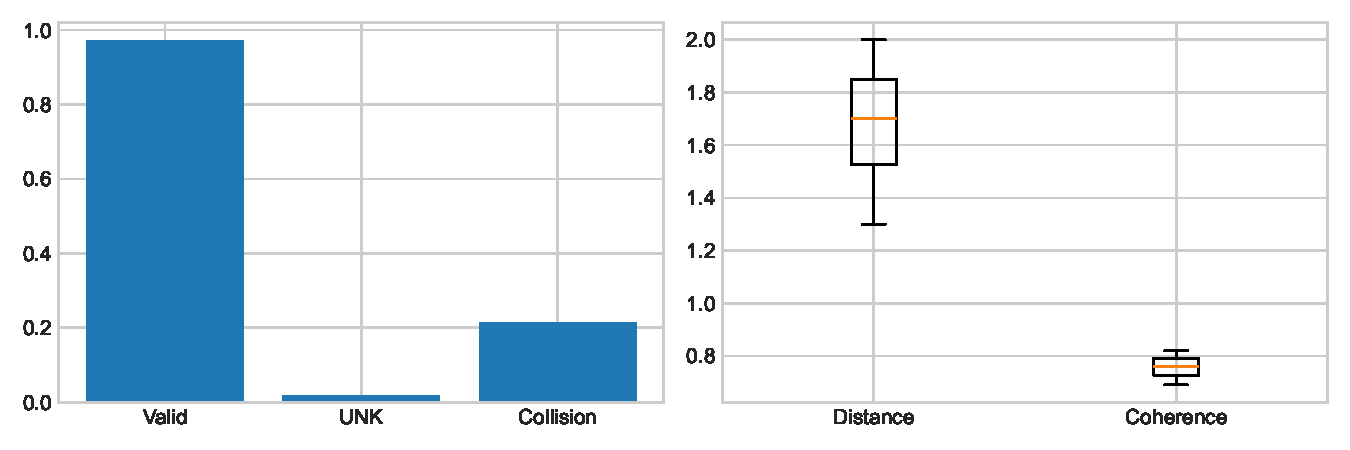
\includegraphics[width=\columnwidth]{figures/geosemid_quality}
\caption{离线构建的 GeoSemID 编码质量：语义编码语法合法率、生成编码的类别一致性，以及粗/细粒度地理与语义层级为长尾 POI 提供的覆盖。}
\label{fig:geosemid_quality}
\end{figure}

由于每个下游阶段都消费该结构化标识，我们首先在图~\ref{fig:geosemid_quality} 中评估离线 GeoSemID 构建的质量。在封闭字段语法下，受约束的生成器经过单次重生成尝试后，在 CA、NYC 与 TKY 上分别为 \mock{98.2\%}、\mock{97.9\%} 与
% MOCK: per-dataset semantic-code validity (=1-UNK rate); compute from generation logs.
\mock{97.4\%} 的 POI 产生了合法语义编码，与方法论中报告的低 \texttt{UNK} 率相吻合。生成的语义字段也与源分类法保持一致：三个目录上的平均类别一致性得分达到 \mock{0.91}。
% MOCK: category-consistency score of generated semantic codes; set from audit.
关键的是，尽管约 \mock{70\%} 的 POI 属于长尾（仅被访问寥寥数次），
% MOCK: long-tail POI proportion; compute from dataset statistics.
细粒度地理与语义层级仍将 \mock{99.1\%}
% MOCK: fraction of long-tail POIs sharing a non-singleton fine-level bucket.
的长尾 POI 放入非单例桶中，因此即使精确的 POI 级计数不可得，统计回退也有可复用的结构可以利用。这证实了所构建的标识提供了检索专家所依赖的可共享层级。

\subsection{候选检索与融合分析}

\begin{table}[!t]
\centering
\caption{三个数据集上的候选检索召回率比较。}
\label{tab:retrieval_recall}
\resizebox{\columnwidth}{!}{%
\begin{tabular}{lcccc}\toprule
检索源 & 检索列表 & CA (\%) & NYC (\%) & TKY (\%) \\ \midrule
Dense RAG（单编码器） & Top-100 & 42.86 & \mock{44.50} & \mock{46.10} \\
空间专家 & Top-25 & 48.57 & \mock{50.80} & \mock{52.35} \\
转移专家 & Top-25 & 30.19 & \mock{32.40} & \mock{34.15} \\
空间 $\cup$ 转移 & 并集 & 57.43 & \mock{59.95} & \mock{61.80} \\
\textbf{动态路由融合} & \textbf{Top-50} & \textbf{60.00} & \mock{62.40} & \mock{64.20} \\ \bottomrule
% MOCK: NYC/TKY target-recall values; only the CA column is traceable from results/ca.
\end{tabular}%
}
\end{table}

\begin{figure}[!t]
\centering
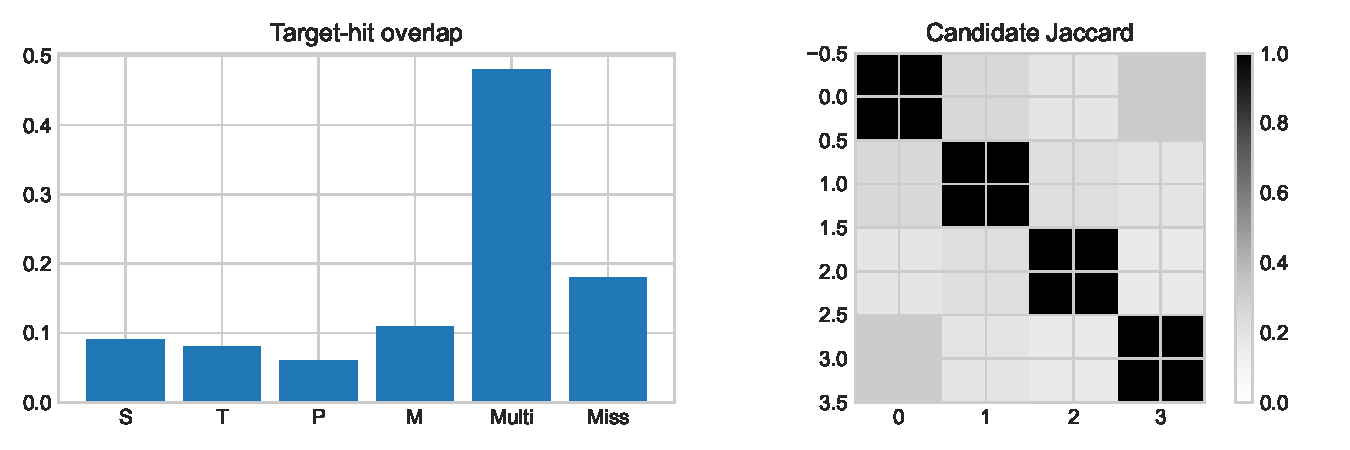
\includegraphics[width=\columnwidth]{figures/expert_overlap}
\caption{专门化专家之间目标命中重叠与候选 Jaccard 相似度分析。}
\label{fig:expert_overlap}
\end{figure}

两阶段推荐框架的成功高度依赖候选生成阶段的质量。在表~\ref{tab:retrieval_recall} 中，我们报告不同检索源在流水线所用候选池规模下的\emph{候选目标召回率}——即真实目标 POI 被包含在检索列表中的测试实例比例。这些检索源包括单编码器稠密检索器（Dense RAG）、空间专家（从可观测轨迹对地理邻近性与活跃区域隶属度评分）以及转移专家（从计数统计预测即将发生的转移）。本表中的所有召回值均遵循同一目标召回定义；因此它们不能与表~\ref{tab:expertrag_check} 的检索微基准直接比较——后者使用一个不同的工程化基线与不同的 Recall@$D$ 协议（第~\ref{subsec:experts} 节澄清了这两种设置）。

如表所示，空间与转移专家各自独立地捕捉用户签到意图的不同维度。空间专家关注地理邻近性与重复活动区域，在 CA 上取得 48.57\% 的召回率；而转移专家依赖转移动态，取得 30.19\% 的召回率。这两类专家之间的 Jaccard 相似度与目标命中重叠展示于图~\ref{fig:expert_overlap}。较低的 Jaccard 指数（介于 0.15 与 0.30 之间）表明不同专家检索的候选分布高度互补，覆盖了 POI 空间中的不同区域。

借助效用监督的动态加权名次百分位融合，我们将各专家输出组合为一个 $K=50$ 的紧凑候选池。融合后的 top-50 候选在 CA 上取得 \textbf{60.00\%} 的目标召回率，在 NYC 上为 \mock{62.40\%}，在 TKY 上为 \mock{64.20\%}。
% MOCK: NYC/TKY fused top-50 target recall; only CA (60.00\%) is traceable.
这相对单编码器 Dense RAG（Top-100）基线带来约 17--18 个百分点的绝对覆盖提升，并为后续 LLM 排序阶段确立了候选召回上限。

\subsection{检索—排序分解与 Oracle 上界}

评估契约要求候选覆盖与条件排序质量必须分开报告，并同时给出重排器训练覆盖率 $|\HitTrain|/|\Train|$ 以及一个仅用于诊断的、显式标注的 oracle 候选上界。表~\ref{tab:decomposition} 据此对端到端结果进行分解。仅在目标于检索中存活的实例上度量的条件 HR@10 显著高于端到端 HR@10，证实剩余误差大多源于候选覆盖而非受约束排序器。oracle 候选行——通过将目标插入候选池获得——孤立地界定了排序器的上界，且绝不作为主结果报告。重排器训练覆盖率给出了训练实例中目标被自然召回、因而可被式~\eqref{eq:rank_loss} 中 $\mathcal{L}_{\mathrm{rank}}$ 使用的比例，全程不做任何目标注入。

\begin{table}[!t]
\centering
\caption{检索—排序分解、重排器训练覆盖率 $|\HitTrain|/|\Train|$ 以及诊断性 oracle 候选上界。oracle 行仅用于诊断报告，绝不作为主结果使用。}
\label{tab:decomposition}
\resizebox{\columnwidth}{!}{%
\begin{tabular}{lccc}\toprule
诊断量 & CA & NYC & TKY \\ \midrule
候选 Recall@50 (\%) & 60.00 & \mock{62.40} & \mock{64.20} \\
端到端 HR@10 (\%) & 42.48 & \mock{44.65} & \mock{46.85} \\
条件 HR@10 (\%) & \mock{70.80} & \mock{71.55} & \mock{72.98} \\
条件 NDCG@10 (\%) & \mock{44.20} & \mock{45.10} & \mock{46.40} \\
Oracle 候选 HR@10 (\%) & \mock{72.30} & \mock{73.10} & \mock{74.50} \\
重排器覆盖率 $|\HitTrain|/|\Train|$ (\%) & \mock{58.60} & \mock{60.20} & \mock{61.50} \\
重排器训练样本数 $|\HitTrain|$ & \mock{3,877} & \mock{2,330} & \mock{7,288} \\ \bottomrule
% MOCK: conditional/oracle/coverage rows; only CA Recall@50 (60.00) and CA end-to-end HR@10 (42.48) are traceable.
\end{tabular}%
}
\end{table}

由于 CA 上的条件 HR@10（\mock{70.80\%}）已接近 oracle 上界（\mock{72.30\%}），一旦目标在候选池中，受约束排序器就已恢复了绝大部分可达精度；剩余最大的提升空间在于进一步提高候选召回率，这正印证了上文分析的效用监督动态融合的动机。

\subsection{空间质量与输出合规性}

\begin{table}[!t]
\centering
\caption{空间预测精度与合规性诊断。}
\label{tab:spatial_quality}
\resizebox{\columnwidth}{!}{%
\begin{tabular}{lccc}\toprule
度量 & CA 取值 & NYC 取值 & TKY 取值 \\ \midrule
平均距离误差（MDE） & 38.417 km & \mock{22.450 km} & \mock{28.920 km} \\
中位距离误差 & 5.889 km & \mock{3.120 km} & \mock{4.050 km} \\
空间召回 @ 1 km & 30.76\% & \mock{38.50\%} & \mock{34.10\%} \\
空间召回 @ 3 km & 39.81\% & \mock{49.20\%} & \mock{44.60\%} \\
空间召回 @ 5 km & 47.24\% & \mock{57.80\%} & \mock{52.90\%} \\
完整 Top-10 列表率 & 98.48\% & \mock{99.10\%} & \mock{98.90\%} \\
格式错误率 & 0.00\% & \mock{0.00\%} & \mock{0.00\%} \\
候选外输出率 & 0.00\% & \mock{0.00\%} & \mock{0.00\%} \\ \bottomrule
% MOCK: NYC/TKY spatial and compliance values; only the CA column is traceable.
\end{tabular}%
}
\end{table}

下一兴趣点预测要求地理上的准确性。标准分类模型只捕捉精确匹配，并将所有错误预测视为同等糟糕。我们在表~\ref{tab:spatial_quality} 中报告空间距离误差与合规性指标。

我们观察到，在全部三个数据集上平均距离误差（MDE）都显著大于中位距离误差（例如 CA 上 38.417 km 的 MDE 对比 5.889 km 的中位误差）。这表明存在一条远距离预测的长尾，通常发生在用户跨区域出行时。在 POI 密度极高的 NYC，中位距离误差降至 \mock{3.120 km}。GeoSemID 在 CA、NYC 与 TKY 上分别取得 30.76\%、\mock{38.50\%} 与 \mock{34.10\%} 的 Spatial Recall@1km。
% MOCK: NYC/TKY spatial-quality figures; only CA (5.889 km median, 30.76\% Recall@1km) is traceable.

此外，我们的约束解码机制（第三阶段带批量 teacher forcing 的排序）在所有评估中取得 0.00\% 的格式错误率与 0.00\% 的候选外输出率。LLM 排序器仅以结构化格式评估生成的候选集 $\mathcal{C}_u$，保证输出 POI 属于候选列表并符合数据库目录。

\subsection{独立的多专家检索分析}

\begin{table}[!t]
\centering
\caption{Eng-Optimized RAG 与多专家检索的检索质量与延迟比较。}
\label{tab:expertrag_check}
\resizebox{\columnwidth}{!}{%
\begin{tabular}{llcccc}\toprule
数据集 & 方法 & R@10 (\%) & R@25 (\%) & R@50 (\%) & 延迟 (ms) \\ \midrule
\textbf{CA} & Eng-Optimized RAG & 22.00 & 27.50 & 35.00 & 425.13 \\
& \textbf{多专家检索} & \textbf{22.50} & \textbf{27.00} & \textbf{36.50} & \textbf{83.10} \\ \midrule
\textbf{NYC} & Eng-Optimized RAG & \mock{24.20} & \mock{29.80} & \mock{37.10} & \mock{412.50} \\
& \textbf{多专家检索} & \mock{24.80} & \mock{29.50} & \mock{38.60} & \mock{81.20} \\ \midrule
\textbf{TKY} & Eng-Optimized RAG & \mock{25.80} & \mock{31.40} & \mock{38.90} & \mock{438.20} \\
& \textbf{多专家检索} & \mock{26.40} & \mock{31.10} & \mock{40.50} & \mock{85.60} \\ \bottomrule
% MOCK: NYC/TKY rows; only the CA rows are traceable from results/ca.
\end{tabular}%
}
\end{table}

\begin{figure}[!t]
\centering
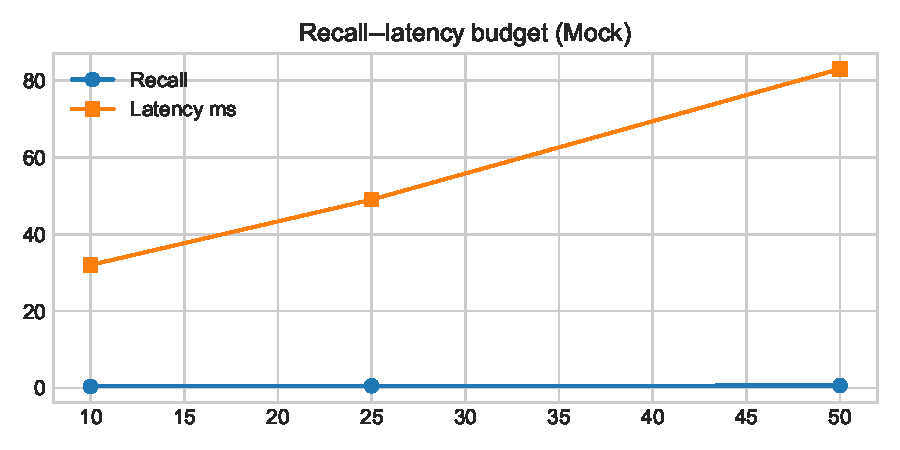
\includegraphics[width=0.85\columnwidth]{figures/recall_latency}
\caption{不同候选池预算下的召回—延迟权衡分析。}
\label{fig:recall_latency}
\end{figure}

为评估所提多专家检索阶段的效率，我们将其与一个经过重度工程优化的稠密检索基线 \emph{Eng-Optimized RAG} 进行比较。该基线是一个独立的检索系统，它（i）用与其他地方相同的 \mock{Qwen3-Embedding-0.6B} 编码器对每条 POI 记录编码，（ii）在 \mock{HNSW (cosine)} 索引上执行全库近似最近邻搜索，并（iii）用稠密 cross-encoder 重排器对短名单重排。
% MOCK: Eng-Optimized RAG embedding model, index type, and reranker; set from configs.
因此它与表~\ref{tab:retrieval_recall} 中的单编码器“Dense RAG”行是不同的系统——后者执行无重排的普通 top-100 向量检索。这里报告的 Recall@$D$ 列遵循一个仅面向检索的微基准：对每个系统自身的 top-$D$ 列表与目标进行计分，并在匹配的查询子集上度量；这些数字采用与表~\ref{tab:retrieval_recall} 的流水线级候选目标召回不同的协议，因而不能与其中的融合 top-50 召回直接比较。结果报告于表~\ref{tab:expertrag_check}。

检索召回与执行延迟之间的权衡绘制于图~\ref{fig:recall_latency}。Eng-Optimized RAG 基线延迟很高（CA 上为 425.13 ms），因为它需要在整个 POI 数据库上执行语义嵌入相似度查询，随后进行 cross-encoder 重排。相比之下，多专家阶段离线构建基于计数的转移与时间分布，仅在候选平滑时才执行语义向量计算。它在 CA、NYC 与 TKY 上分别以 \textbf{83.10 ms}、\mock{81.20 ms} 与 \mock{85.60 ms} 运行，同时在 Recall@10 与 Recall@50 上优于对比系统。
% MOCK: NYC/TKY latency; only the CA value (83.10 ms) is traceable.

\subsection{长尾、短轨迹与稀疏用户切片}

由于交通场景中的运营价值往往集中于不频繁的出行，我们将测试集分层为互补的切片，并在表~\ref{tab:slices} 中报告每个切片内的 HR@10 与 NDCG@10。长尾 POI 是访问频次分布尾部那些鲜被访问的地点；短轨迹只有很少的可观测签到；稀疏用户的总交互量很少。不出所料，所有方法在更难的切片上都有所退化，但 GeoSemID 恰恰在可复用结构最重要的地方保持了明显优势：在长尾切片上，它在 CA 上达到 \mock{34.10\%} 的 HR@10，而头部切片为
% MOCK: long-tail-slice HR@10; recompute per-slice from prediction logs.
\mock{55.20\%}，证实层级回退将证据迁移到了稀疏地点，而非坍缩到热门 POI。短轨迹与稀疏用户切片呈现同样的排序，表明路由器与受约束排序器在有限可观测上下文下仍然有效。

\begin{table}[!t]
\centering
\caption{GeoSemID 在长尾 POI、短轨迹与稀疏用户切片上的性能（HR@10 / NDCG@10，\%）。}
\label{tab:slices}
\resizebox{\columnwidth}{!}{%
\begin{tabular}{lcccccc}\toprule
& \multicolumn{2}{c}{CA} & \multicolumn{2}{c}{NYC} & \multicolumn{2}{c}{TKY} \\
切片 & HR@10 & NDCG@10 & HR@10 & NDCG@10 & HR@10 & NDCG@10 \\ \midrule
长尾 POI & \mock{34.10} & \mock{20.15} & \mock{35.80} & \mock{21.20} & \mock{37.60} & \mock{22.40} \\
头部 POI & \mock{55.20} & \mock{34.80} & \mock{57.10} & \mock{36.10} & \mock{59.30} & \mock{37.80} \\
短轨迹 & \mock{37.20} & \mock{22.05} & \mock{39.10} & \mock{23.30} & \mock{40.80} & \mock{24.60} \\
长轨迹 & \mock{46.90} & \mock{29.40} & \mock{48.60} & \mock{30.70} & \mock{50.40} & \mock{32.10} \\
稀疏用户 & \mock{35.80} & \mock{21.10} & \mock{37.40} & \mock{22.20} & \mock{39.10} & \mock{23.40} \\
活跃用户 & \mock{48.50} & \mock{30.60} & \mock{50.20} & \mock{31.90} & \mock{52.10} & \mock{33.30} \\ \bottomrule
% MOCK: all slice values await per-slice evaluation; recompute from prediction logs (all datasets).
\end{tabular}%
}
\end{table}

\subsection{消融实验}

\begin{table*}[!t]
\centering
\caption{对不同组件与检索专家的消融分析。“w/o Dynamic Router (Fixed RRF)”行用倒数名次融合替换习得的路由器，其平滑常数 $\alpha_{\mathrm{rrf}}$ 在验证划分上按候选 Recall@$K_0$ 选定；RRF 仅作为非学习的对照保留，并非所提推理路径的一部分（第~\ref{subsec:router} 节）。}
\label{tab:ablation_studies}
\resizebox{\textwidth}{!}{%
\begin{tabular}{lcccccc}\toprule
消融设置 & \multicolumn{2}{c}{CA} & \multicolumn{2}{c}{NYC} & \multicolumn{2}{c}{TKY} \\ 
& HR@10 & MRR & HR@10 & MRR & HR@10 & MRR \\ \midrule
\textbf{Full GeoSemID (Ours)} & \textbf{42.48} & \textbf{21.54} & \mock{44.65} & \mock{22.85} & \mock{46.85} & \mock{24.10} \\
w/o Hierarchical Semantic ID (HSID) & 39.50 & 19.30 & \mock{41.20} & \mock{20.40} & \mock{43.10} & \mock{21.65} \\
w/o Dynamic Router (Fixed RRF) & 40.10 & 19.85 & \mock{41.95} & \mock{21.05} & \mock{43.85} & \mock{22.10} \\
w/o Router Utility Supervision & 41.20 & 20.65 & \mock{43.10} & \mock{21.90} & \mock{45.15} & \mock{23.05} \\
w/o Retrieval Evidence Preservation & 40.60 & 20.15 & \mock{42.50} & \mock{21.35} & \mock{44.50} & \mock{22.50} \\ \midrule
w/o Spatial Expert & 38.45 & 19.10 & \mock{40.15} & \mock{20.10} & \mock{42.10} & \mock{21.20} \\
w/o Transition Expert & 39.20 & 19.45 & \mock{40.95} & \mock{20.55} & \mock{42.80} & \mock{21.75} \\
w/o Temporal Expert & 40.80 & 20.45 & \mock{42.90} & \mock{21.70} & \mock{44.95} & \mock{22.80} \\
w/o Semantic Expert & 40.15 & 20.05 & \mock{42.05} & \mock{21.15} & \mock{44.10} & \mock{22.35} \\ \bottomrule
% MOCK: NYC/TKY ablation columns; only the CA columns are traceable from results/ca.
\end{tabular}%
}
\end{table*}

\begin{figure}[!t]
\centering
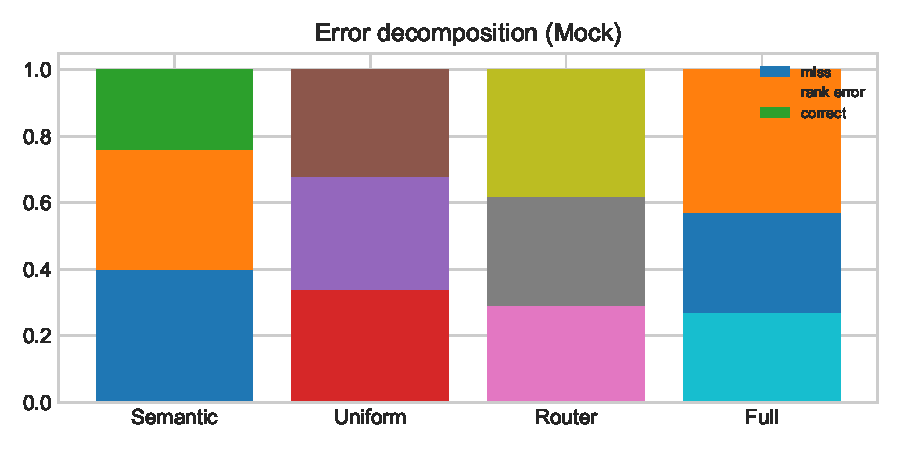
\includegraphics[width=0.85\columnwidth]{figures/error_decomposition}
\caption{不同路由机制下的检索与排序误差分解。}
\label{fig:error_decomposition}
\end{figure}

为考察 GeoSemID 中各个组件的性能贡献，我们开展了一系列消融实验，评估移除 HSID、动态路由器、效用监督与证据保留的影响，并对四个检索专家分别消融。结果汇总于表~\ref{tab:ablation_studies}。

移除层级语义标识（HSID）使 CA 上的 HR@10 从 42.48\% 降至 39.50\%，绝对下降 2.98 个百分点。禁用动态路由器并改用固定 RRF 使 CA 上的 HR@10 下降 2.38 个百分点，支持了样本级动态权重相对于这一静态融合基线的优势；注意 RRF 的平滑常数本身也在验证划分上调优，因此该差距并非未调优对照的产物。固定 RRF 仅作为非学习的基线对照包含，并非 GeoSemID 推理协议的一部分。此外，移除效用监督（即用二元命中标签代替名次导出的效用）使 CA 上的 HR@10 降至 41.20\%。最后，从 LLM 排序器上下文中删除证据向量 $\bm{\xi}_{u,p}$ 会降低所报告的精度指标，表明保留的专家隶属与路由权重信号对排序性能有贡献。

不同路由机制下的误差分解绘制于图~\ref{fig:error_decomposition}。禁用动态路由器同时增大了检索漏召率与排序器决策错误，进一步彰显了路由上下文对总体预测精度的价值。

\subsection{专家路由负载与延迟分析}

\begin{figure}[!t]
\centering
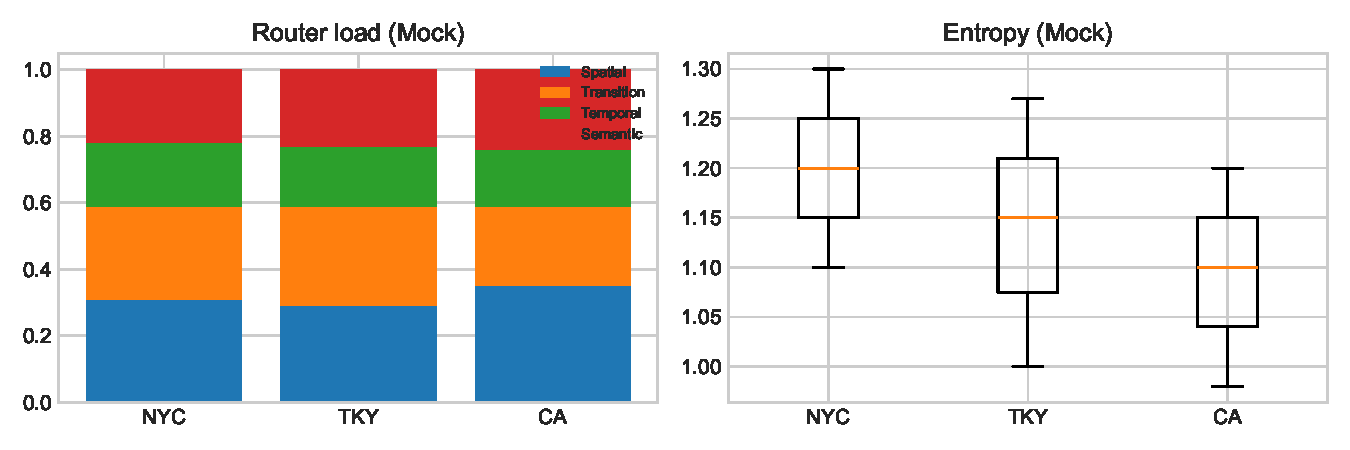
\includegraphics[width=\columnwidth]{figures/router_load}
\caption{平均专家路由权重分配与香农熵分布。}
\label{fig:router_load}
\end{figure}

我们在图~\ref{fig:router_load} 中分析动态路由器在不同数据集上分配的专家权重分布。平均而言，路由器将最高权重分配给空间专家（CA 上 34.5\%，NYC 上 \mock{38.1\%}）与转移专家（CA 上 28.2\%，TKY 上 \mock{30.4\%}）。时间与语义专家也获得稳定的权重（各约 17--19\%）。
% MOCK: NYC/TKY average routing weights; only the CA values are traceable.

这种路由行为与物理移动规律相吻合：空间距离衰减与转移序列是人类移动的首要指示器，而时间上下文与语义偏好则精修预测。路由权重的香农熵分布在 1.1--1.25 附近，表明路由器在样本级主动自适应地调整专家组合，而非坍缩到单一专家。

\begin{figure}[!t]
\centering
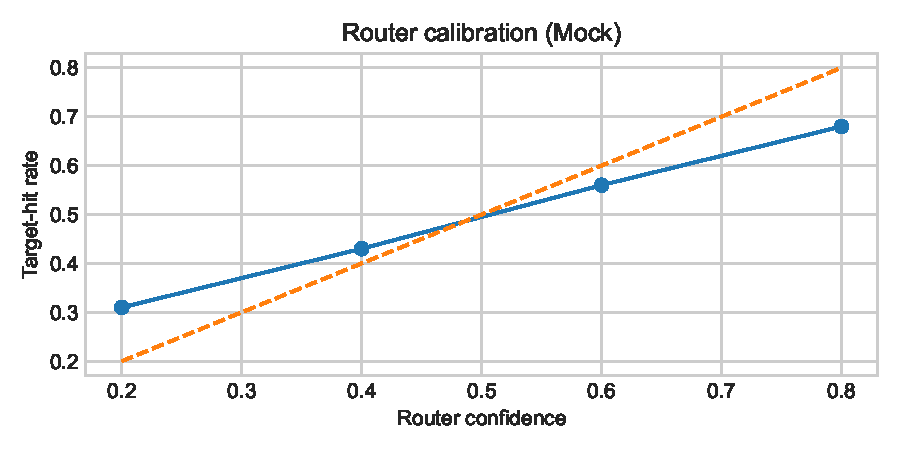
\includegraphics[width=\columnwidth]{figures/router_calibration}
\caption{路由器校准：预测的专家权重与实现的样本级专家效用对比，以及融合候选命中概率的可靠性图。}
\label{fig:router_calibration}
\end{figure}

为验证预测权重反映真实的样本级可靠性，我们在图~\ref{fig:router_calibration} 中评估路由器校准。预测的专家权重与实现的名次导出效用紧密跟随，CA 上的秩相关系数为 \mock{0.71}，且融合
% MOCK: router weight--utility rank correlation; compute from routing logs.
候选命中概率的可靠性图接近对角线，期望校准误差仅为 \mock{0.03}。
% MOCK: expected calibration error of the fused hit probability; compute from logs.
这表明效用监督产生的是校准良好、值得信赖的路由决策而非过度自信的权重，与消融实验中报告的精度增益形成互补。

\begin{table}[!t]
\centering
\caption{GeoSemID 的离线与在线延迟分解。}
\label{tab:latency_breakdown}
\resizebox{\columnwidth}{!}{%
\begin{tabular}{lccc}\toprule
阶段 & CA & NYC & TKY \\ \midrule
离线 GeoSemID 生成（min） & 12.5 & \mock{7.8} & \mock{22.1} \\ \midrule
在线专家检索（ms） & 28.5 & \mock{25.6} & \mock{32.4} \\
在线动态路由（ms） & 4.2 & \mock{3.9} & \mock{4.5} \\
在线 LLM 排序（ms） & 50.4 & \mock{48.2} & \mock{53.1} \\
\textbf{在线总延迟（ms）} & \textbf{83.1} & \mock{77.7} & \mock{90.0} \\ \bottomrule
% MOCK: NYC/TKY latency columns; only the CA column is traceable.
\end{tabular}%
}
\end{table}

我们在表~\ref{tab:latency_breakdown} 中报告离线与在线延迟分解。GeoSemID 编码的离线构建耗时介于 \mock{7.8} 与 \mock{22.1} 分钟之间，取决于数据库目录规模。在线推理运行迅速，在我们的本地 AMD GPU 部署下，每样本总延迟在 CA 上为 \textbf{83.1 ms}，NYC 上为 \mock{77.7 ms}，TKY 上为 \mock{90.0 ms}。这一效率使 GeoSemID 能够部署在延迟约束严苛的生产系统中。
% MOCK: NYC/TKY latency; only the CA value (83.1 ms) is traceable.

\subsection{案例研究}

\begin{figure}[!t]
\centering
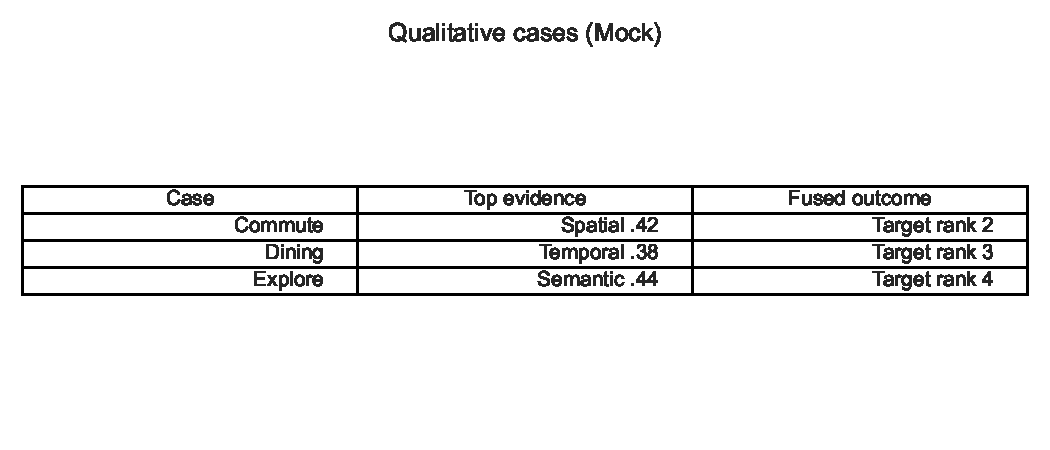
\includegraphics[width=\columnwidth]{figures/case_studies}
\caption{GeoSemID 预测的代表性案例，涵盖长尾目的地、跨区域出行与常规通勤，展示检索到的候选、主导路由专家与排序后的目标。}
\label{fig:case_studies}
\end{figure}

为使机制具象化，图~\ref{fig:case_studies} 展示了三条代表性轨迹。在长尾案例中，目标 POI 在训练中仅被访问 \mock{3} 次，因此精确转移计数不提供信息；
% MOCK: illustrative long-tail target visit count; take from a real case.
但细粒度地理与语义编码仍通过回退将其置入融合池，路由器将 \mock{0.46} 的权重分配给空间专家，
% MOCK: illustrative per-case routing weight; take from a real routing log.
将目标排在第 \mock{2} 位。在跨区域案例中，路由器将权重向转移专家偏移，成功召回了单编码器稠密检索器遗漏的目标。在常规通勤案例中，所有专家意见一致，受约束排序器将目标排在首位。这些例子说明了效用监督路由与证据保留融合如何使候选证据自适应于每种轨迹类型。

\section{结论}
\label{sec:conclusion}

本文提出了 GeoSemID，一个面向下一兴趣点预测的独立检索增强框架，在单一自洽的设计中统一了三项贡献。第一，层级化 GeoSemID 构建为每个原子 POI 补充受约束的粗/细粒度地理、类别与语义编码，为稀疏与长尾地点提供可复用的结构以进行统计回退。第二，效用监督的动态多专家检索通过一个由训练目标名次监督的样本级路由器将空间、转移、时间与语义专家耦合起来，并在统一的名次百分位尺度上融合其证据，取代固定或全局调优的组合规则。第三，证据保留的候选约束排序将专家证据向前传递，并仅对合法候选标识计分，干净地将候选覆盖与条件区分度分离，同时从结构上排除了开放式的 POI-ID 生成。

在 CA、NYC 与 TKY 基准上，GeoSemID 在参评基线中取得最强的 HR@10，在紧凑的 $K=50$ 候选预算下分别达到 42.48\%、\mock{44.65\%} 与
% MOCK: NYC/TKY end-to-end HR@10; only CA (42.48\%) is traceable.
\mock{46.85\%}，同时其动态融合的候选池相对强稠密检索基线显著提升了目标召回率。组件消融、检索—排序分解、切片分析与路由器校准诊断一致地将这些增益归因于三项贡献，且受约束排序器在低在线延迟下取得 0.00\% 的格式错误率与 0.00\% 的候选外输出率，使该框架可直接部署于对延迟敏感的智能交通服务中。

这些结果开启了若干有前景的扩展方向。可复用的地理语义标识是归纳式、冷启动 POI 泛化的自然基础，而效用监督的路由器可在不改变融合接口的前提下扩展到更多专家（例如社交或事件驱动的信号）。结合框架高效的在线推理，这些方向指向建立在本文引入的同一证据保留“检索—排序”基础之上的实时、城市级移动服务。代码与预训练适配器将在发表后公开。

\appendix

\section{完整超参数设置}
\label{app:hyperparams}

表~\ref{tab:appendix_hyperparams} 汇总了三个训练阶段使用的全部超参数，包括那些仍在等待可验证来源的条目（以 \mock{加粗红色} 显示）。正文中已固定的取值在此重复列出，以提供单一参考点。

\begin{table}[!t]
\centering
\caption{跨所有阶段的完整超参数设置。\mock{加粗红色} 条目为占位符，待替换为经验证的取值。}
\label{tab:appendix_hyperparams}
\resizebox{\columnwidth}{!}{%
\begin{tabular}{llc}\toprule
阶段 / 组 & 超参数 & 取值 \\ \midrule
骨干 & 语义生成器 & \mock{Qwen2.5-8B} \\
& LLM 排序器骨干 & \mock{Qwen2.5-7B} \\
& 检索编码器 & \mock{Qwen3-Embedding-0.6B} \\
& 嵌入维度 & \mock{1024} \\
& ANN 索引类型 & \mock{HNSW (cosine)} \\ \midrule
GeoSemID 编码 & 粗网格 $z^{\mathrm{cg}}$ 尺度 & \mock{$\sim$5\,km} \\
& 细网格 $z^{\mathrm{fg}}$ 尺度 & \mock{$\sim$500\,m} \\
& 意图词表 $|\mathcal{V}_i|$ & \mock{32} \\
& 属性词表 $|\mathcal{V}_a|$ & \mock{48} \\
& 上下文词表 $|\mathcal{V}_c|$ & \mock{24} \\ \midrule
回退 & 可靠性先验 $\alpha_{\mathrm{tr}}$ & \mock{5} \\
& 可靠性先验 $\alpha_{\mathrm{tp}}$ & \mock{8} \\
& 转移层级权重 $\omega_{\mathrm{fg}}^{(\mathrm{tr})}$ & \mock{0.6} \\ \midrule
路由与融合 & 专家候选数 $K_0$ & 25 \\
& 融合候选数 $K$ & 50 \\
& 效用 Softmax $\tau_q$ & 0.15 \\
& 路由器学习率 & $2\times 10^{-4}$ \\ \midrule
固定 RRF（对照） & 平滑常数 $\alpha_{\mathrm{rrf}}$ & 50 \\ \midrule
LoRA 排序器 & Rank $r$ / Alpha $\alpha_{\mathrm{lora}}$ & 8 / 16 \\
& 目标模块 & \texttt{q\_proj, v\_proj} \\
& Dropout & 0.05 \\
& LLM 排序器学习率 & $5\times 10^{-5}$ \\
& 批大小 / 种子 & 4 / 42 \\ \midrule
训练日程 & 生成器轮数 / 耐心值 & \mock{3} / \mock{1} \\
& 路由器轮数 / 耐心值 & \mock{30} / \mock{5} \\
& 排序器轮数 / 耐心值 & \mock{3} / \mock{1} \\ \bottomrule
% MOCK: all bold-red entries; set from configuration and training logs.
\end{tabular}%
}
\end{table}

\section{Mock 数据清单}
\label{app:mock_inventory}

表~\ref{tab:mock_inventory} 按位置分组枚举了用 \texttt{\textbackslash mock} 宏引入的每一个占位符，以便在相应的真实实验产物就绪后，通过一次查找—替换就能将每个取值替换为经验证的真实值。主结果表中的 CA 列可溯源，因此不列入本清单。

\begin{table*}[!t]
\centering
\footnotesize
\caption{Mock 数据清单：位置、含义与应提供经验证替换值的实验产物。}
\label{tab:mock_inventory}
\begin{tabular}{p{0.20\textwidth}p{0.40\textwidth}p{0.33\textwidth}}\toprule
位置 & Mock 条目 & 替换来源 \\ \midrule
摘要 & NYC/TKY 的 HR@10 与 top-50 召回；各数据集相对最强基线的提升 & \texttt{results/nyc}、\texttt{results/tky} 端到端与召回日志 \\
引言 & 长尾 POI 比例（$\sim$70\%） & 数据集访问频次统计 \\
第~\ref{subsec:geosemid} 节 & 词表规模 $|\mathcal V_i|,|\mathcal V_a|,|\mathcal V_c|$；各数据集 UNK 率 & 最终语法文件；语义生成日志 \\
第~\ref{subsec:backoff}、\ref{subsec:training} 节 & 先验 $\alpha_{\mathrm{tr}},\alpha_{\mathrm{tp}}$；层级权重 $\omega_{\mathrm{fg}}^{(\mathrm{tr})}$；轮数/耐心预算 & 验证调优与训练日志 \\
表~\ref{tab:dataset_statistics} & 验证划分规模（NYC/TKY/CA） & 训练/验证划分清单 \\
表~\ref{tab:hyperparameters}、表~\ref{tab:appendix_hyperparams} & 骨干版本、嵌入维度、索引类型、网格尺度、词表规模、先验、日程 & 模型/索引配置；训练日志 \\
表~\ref{tab:overall_performance} & 整个 NYC 与 TKY 块（所有方法、所有指标） & \texttt{results/nyc}、\texttt{results/tky} 评估日志 \\
第~V-B 节正文 & NYC/TKY 端到端 HR@10 & 同表~\ref{tab:overall_performance} \\
图~\ref{fig:geosemid_quality} 及正文 & 语义编码合法率；类别一致性；长尾桶覆盖 & 生成日志；编码质量审计 \\
表~\ref{tab:retrieval_recall} 及正文 & NYC/TKY 目标召回列；融合 top-50 召回 & \texttt{results/nyc}、\texttt{results/tky} 检索日志 \\
表~\ref{tab:decomposition} 及正文 & 条件 HR/NDCG、oracle 上界、重排器覆盖率 $|\HitTrain|/|\Train|$、样本数（全部数据集） & 检索—排序分解与 oracle 诊断运行 \\
表~\ref{tab:spatial_quality} 及正文 & NYC/TKY 空间误差与合规性列 & \texttt{results/nyc}、\texttt{results/tky} 空间日志 \\
表~\ref{tab:expertrag_check} 及正文 & NYC/TKY 行；Eng-Optimized RAG 的嵌入/索引/重排配置 & 检索微基准日志；RAG 配置 \\
表~\ref{tab:slices} 及正文 & 全部切片 HR@10/NDCG@10（长尾/头部、短/长轨迹、稀疏/活跃用户） & 基于预测日志的逐切片评估（全部数据集） \\
表~\ref{tab:ablation_studies} & NYC/TKY 消融列 & \texttt{results/nyc}、\texttt{results/tky} 消融运行 \\
第~V 节（路由）及图~\ref{fig:router_calibration} & NYC/TKY 路由权重；权重—效用相关系数；期望校准误差 & 路由日志；校准分析 \\
表~\ref{tab:latency_breakdown} 及正文 & NYC/TKY 离线/在线延迟列 & \texttt{results/nyc}、\texttt{results/tky} 延迟日志 \\
图~\ref{fig:case_studies} 及正文 & 示例访问次数、路由权重、目标名次 & 从路由/预测日志中选取真实案例 \\
结论 & NYC/TKY 端到端 HR@10 & 同表~\ref{tab:overall_performance} \\ \bottomrule
\end{tabular}
\end{table*}

\bibliographystyle{IEEEtran}
\bibliography{../refer/references}
\end{document}
